\documentclass[serif,mathserif,14pt]{beamer}
%\setbeamercovered{transparent}
\usepackage{listings}
\usepackage{amsmath, amsfonts, epsfig, xspace}
\usepackage{pstricks,pst-node}
\usepackage{multimedia}
\usepackage{beamerthemesplit}
\usetheme{chaosgroup}
% add bulgarian support
\usepackage[utf8]{inputenc}
\usepackage[english,bulgarian]{babel}
\usepackage[T2B]{fontenc}
% include subfigure package
\usepackage[normal,tight,center]{subfigure}
\setlength{\subfigcapskip}{-.5em}

\usepackage{animate}
\usepackage{xmpmulti}

%4 people are authors - \author[Bruce Wayne]{Bruce Wayne \quad Clark Kent\\Peter Parker \quad Alan Scot}
%\addtobeamertemplate{title}{\vskip-0.5ex}{}
\author[Йордан Маджунков]{Йордан Маджунков}
\title[Монте Карло\hspace{2em}\insertframenumber/\inserttotalframenumber]{Въведение в Монте Карло}
%\institute{ 
\includegraphics[width=5cm]{chaoslogo_white.png}}
\date{24 Октомври 2015} %leave out for today's date to be insterted

\usebackgroundtemplate {
\includegraphics[width=\paperwidth, height=\paperheight]{background.jpg}}
\defbeamertemplate*{title page}{customized}[1][] {

\setbeamercolor{author}{fg=write}
\vspace{5cm}
\begin{center}
\usebeamerfont{title} \Large \inserttitle\\
\end{center}
\begin{center}
\usebeamerfont{author} \small \insertauthor
\end{center}

}
\begin{document}

\maketitle

%\section{Introduction}  % add these to see outline in slides
\addtobeamertemplate{frametitle}{\vskip-0.5ex}{}
%\setbeamertemplate{background canvas}[vertical shading][bottom=bottomcolour, middle=middlecolour, top=black]
\setbeamertemplate{background}
{
\includegraphics[width=\paperwidth,height=\paperheight]{backgroud_new.png}}
\lstset{language=C++,
        basicstyle=\ttfamily,
        keywordstyle=\color{green}\ttfamily,
        stringstyle=\color{red}\ttfamily,
        commentstyle=\color{blue}\ttfamily,
        morecomment=[l][\color{magenta}]{\#}
}
\renewcommand*{\thesubfigure}{}

\begin{frame}
  \frametitle{Въведение}
  Монте Карло алгоритми\pause
  \begin{itemize}
  \item Използват псевдо случай числа\pause
  \item Изчисляват приближено решение\pause
  \item Контрол на точността\pause
  \item Контрол на времето за изпълнение %leave out the \pause on the final item
  \end{itemize}
\end{frame}

\begin{frame}
  \frametitle{Мотивация}
  \pause
  Защото работи\pause
  \begin{itemize}
  \item с ограничени ресурси\pause
  \item върху сложни проблеми\pause
  \item в истинският свят\pause
  \item без алтернатива
  \end{itemize}
\end{frame}
\begin{frame}
  \frametitle{Демотивация}
  Недостатъци на Монте Карло\pause
  \begin{itemize}
  \item Приближен метод\pause
  \item Труден\pause
  \item Бавен 
  \end{itemize}
\end{frame}


\begin{frame}
  \frametitle{История}
  \pause
  \begin{figure}[t]
    \centering
    \subfigure[Stanislaw Ulam]{
    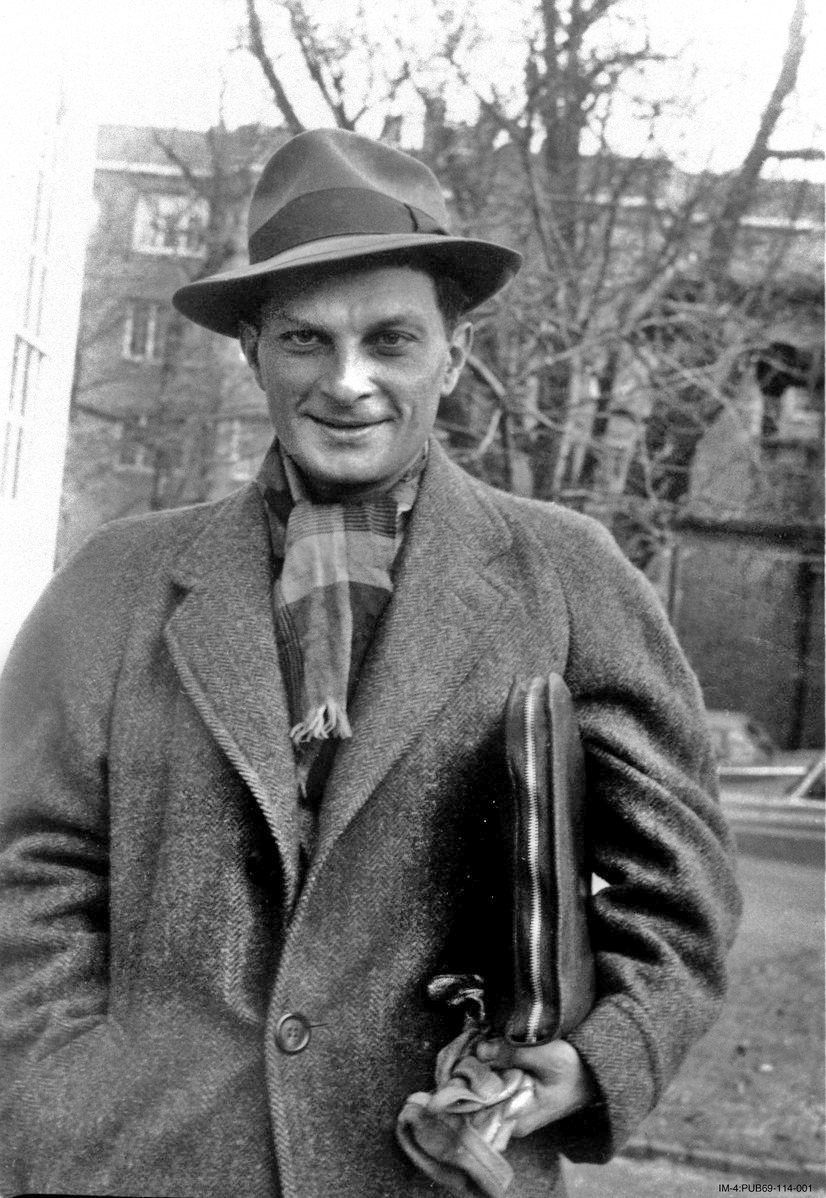
\includegraphics[height=6.0cm]{StanislawUlam.png}}
    \pause
    \subfigure[John von Newmann]{
    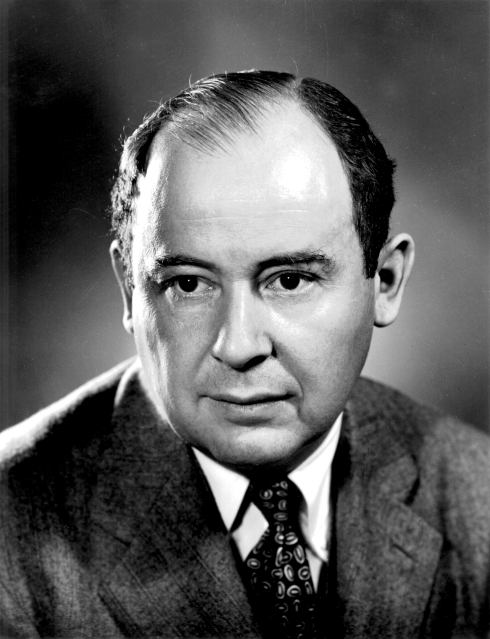
\includegraphics[height=6.0cm]{JohnvonNeumann.png}}
  \end{figure}
\end{frame}

\begin{frame}
  \frametitle{История}
  \begin{figure}[t]
    \centering
    \subfigure[Electronic Numerical Integrator And Computer]{
    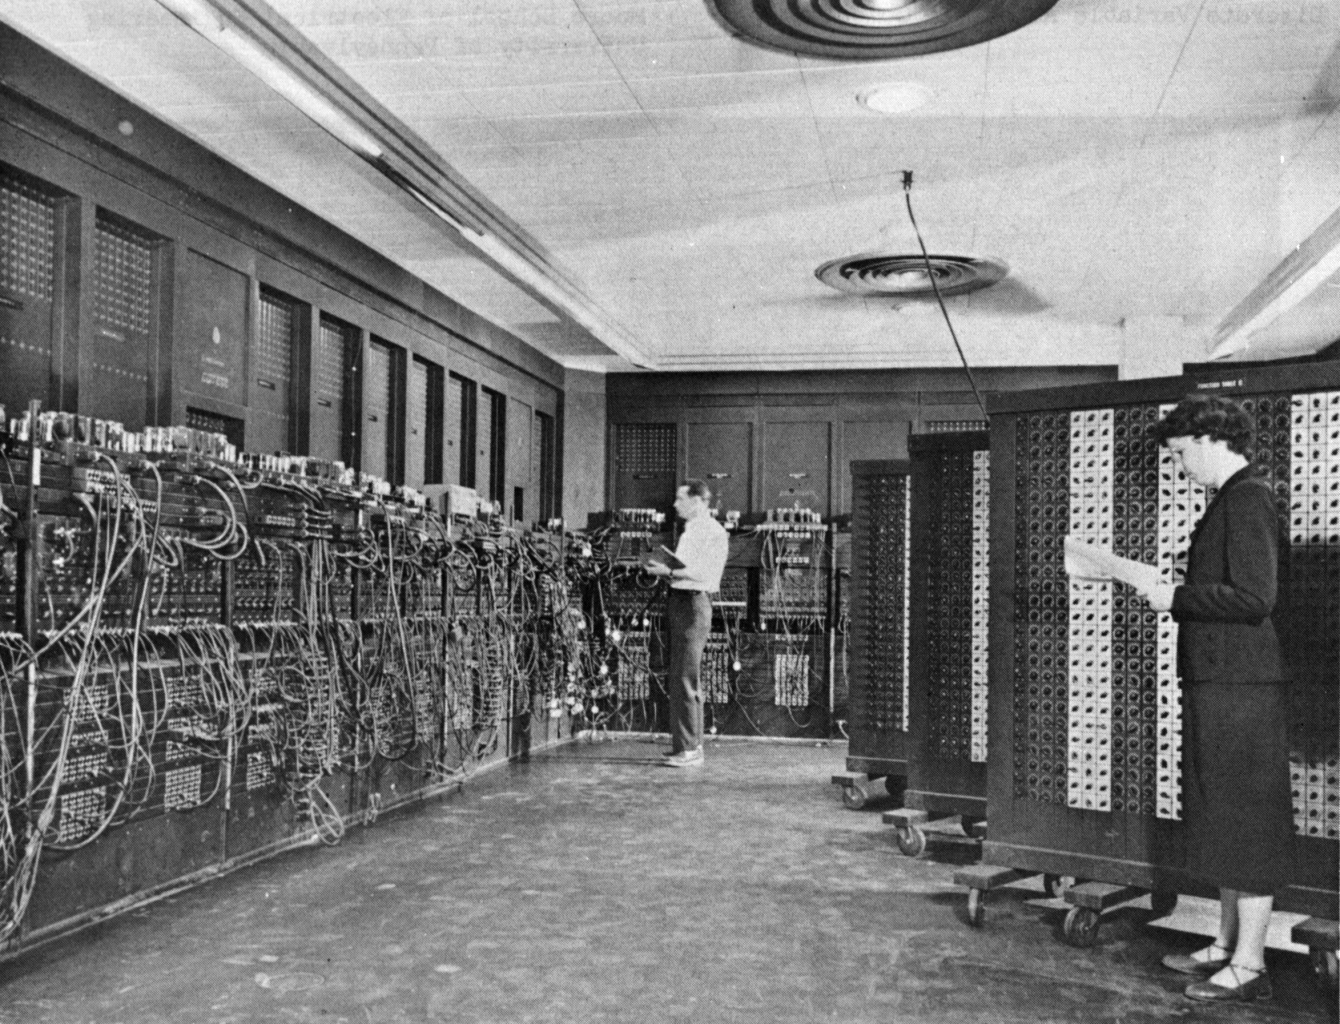
\includegraphics[height=6.5cm]{Eniac.jpg}}
  \end{figure}
\end{frame}
\begin{frame}
  \frametitle{История}
  \begin{figure}[t]
    \centering
    \subfigure[Fat Man]{
    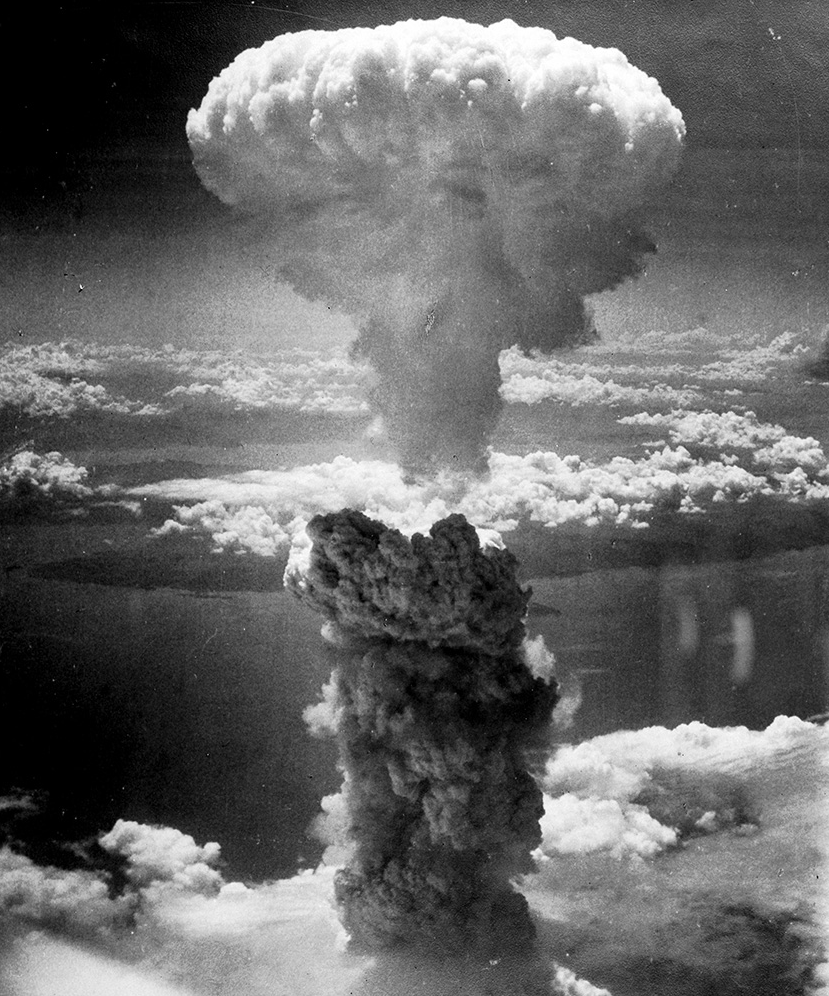
\includegraphics[height=6.5cm]{fatman.png}}
  \end{figure}
\end{frame}


%\begin{frame}
%  \frametitle{Монте Карло интегриране}
%  \begin{equation*}
%  I = \int_{\Omega} h(\mathbf{x}) d \mathbf{x}, \quad
%  x \in \mathbb{R}^d,  \quad
%  V = \int_{\Omega} d \mathbf{x}
%  \end{equation*}
%  \pause
%  \begin{equation*}
%  Q_N = V \frac{1}{N} \sum_{i=1}^N h(\mathbf{x_i}) = V \overline{\mathbf{h}}, \quad 
%  \mathbf{x_1}, \mathbf{x_2}, \dots,  \mathbf{x_N} \in \Omega
%  \end{equation*}
%  \pause
%  \begin{equation*}
%  \mathrm{Var} (h) = \sigma_N^2 = \frac{1}{N-1} \sum_{i=1}^N (h(\mathbf{x_i}) - \overline{\mathbf{h}})^2
%  \end{equation*}
%  \pause
%
%  \begin{equation*}
%  \delta Q_N = \sqrt{\mathrm{Var}(Q_N)} = V \frac{\sigma_n} {\sqrt{N}}
%  \end{equation*}
%
%\end{frame}










\begin{frame}[fragile]
\frametitle{Монте Карло - Дефиниция}
\pause
\begin{lstlisting}
RandomGenerator rng;
for (int i = 0; i < nSamples; i++) {
   x   = sample(rng, ..);
   res = compute(x, ..);
   accumulate(res);
}
reportResults();
\end{lstlisting}
\end{frame}

\begin{frame}[fragile]
\frametitle{Пример}
\pause
\begin{lstlisting}
RandomGenerator rng;
int hits = 0;
for (int i = 0; i < nSamples; i++) {
   float x = rng.getUniform();
   float y = rng.getUniform();
   int res = x*x + y*y < 1.0f ? 1 : 0;
   hits += res;
}
float final = hits * 4.0f / nSamples;
\end{lstlisting}
\end{frame}

\begin{frame}
  \frametitle{$\pi$}
  \vskip-3.5ex
  \begin{figure}[t]
    \animategraphics[height=7.5cm,loop,autoplay]{2}{animated/pi_frame-}{0}{9}
%    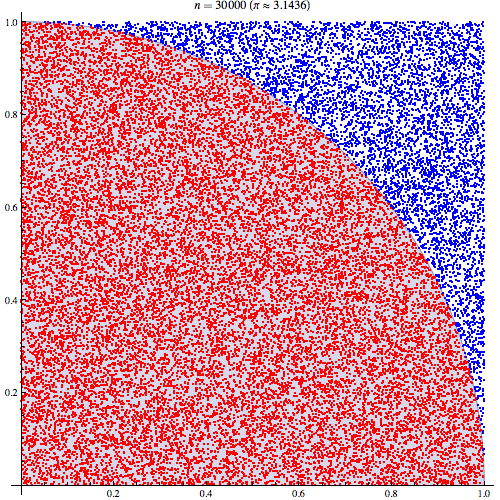
\includegraphics[height=7.5cm]{pi_frame-9.png}
  \end{figure}
\end{frame}

\begin{frame}
  \frametitle{$\pi$ - Монте Карло}
  \begin{equation*}
   h(x,y) = \begin{cases}
        1,& \text{ако } x^2 + y^2 < 1 \\
        0,& \text{иначе}\\
        \end{cases}
  \end{equation*}
  \pause

  \begin{equation*}
    \Omega = x \in [0 .. 1] \times y \in [0 .. 1]
  \end{equation*}
  \pause

  \begin{equation*}
   \int_{\Omega} h(x,y) dx dy = \frac{\pi}{4} \Rightarrow \quad 
  \pause
   \pi = 4 \int_{\Omega} h(x,y) dx dy
  \end{equation*}
\end{frame}


\begin{frame}
  \frametitle{Монте Карло интегриране}
  \begin{equation*}
  I = \int_{\Omega} h(\mathbf{x}) d \mathbf{x} \approx
  \pause
  Q_N = \frac{1}{N} \sum_{i=1}^N h(\mathbf{x_i}) 
  \end{equation*}
\noindent
\makebox[\textwidth]{
%  \includegraphics[height=4.5cm]{animated/montecarlo.png}
  \animategraphics[width=\textwidth,autoplay]{2}{animated/montecarlo_dummy-}{0}{0}
}
\end{frame}

\begin{frame}
  \frametitle{Монте Карло интегриране}
  \addtocounter{framenumber}{-1}
  \begin{equation*}
  I = \int_{\Omega} h(\mathbf{x}) d \mathbf{x} \approx
  Q_N = \frac{1}{N} \sum_{i=1}^N h(\mathbf{x_i}) 
  \end{equation*}
\noindent
\makebox[\textwidth]{
  \animategraphics[width=\textwidth,autoplay]{2}{animated/montecarlo-}{0}{12}
}
\end{frame}


\begin{frame}
  \frametitle{Сходимост}
  \vskip-1.5ex
  \begin{equation*}
   \Delta Q_N = |Q_N - I| \propto \frac{\sqrt{\mathrm{Var}(h)}} {\sqrt{N}} \pause = \frac{\sigma_N} {\sqrt{N}}
  \end{equation*}
  \pause
  \vskip-6.5ex
  \begin{figure}[t]
  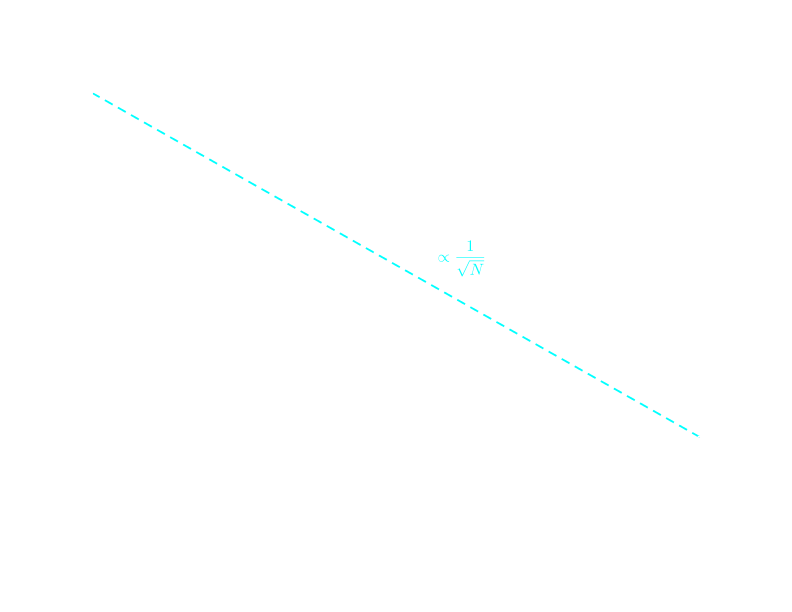
\includegraphics[width=0.7\textwidth]{mc_error2.png}
  \end{figure}
\end{frame}

\begin{frame}
  \frametitle{Сходимост}
  \makebox[\textwidth]{
  \animategraphics[width=\textwidth,autoplay]{2}{animated/montecarlo-}{0}{12}
  }
  \begin{table}
  \begin{tabular}{l | c }
              & Сходимост    \\
  \hline \hline
  Монте Карло & $\mathcal{O}(N^{-1/2})$  \\
      &     \\
  \end{tabular}
  \end{table}
\end{frame}

\begin{frame}
  \frametitle{Сходимост}
  \makebox[\textwidth]{
  \animategraphics[width=\textwidth,autoplay]{2}{animated/trapez-}{0}{12}
  }
  \begin{table}
  \begin{tabular}{l | c }
              & Сходимост    \\
  \hline \hline
  Монте Карло & $\mathcal{O}(N^{-1/2})$  \\
  \pause
  Трапеците   & $\mathcal{O}(N^{-2/s})$    \\
  \end{tabular}
  \end{table}
\end{frame}
%\begin{frame}
%  \frametitle{Сходимост}
%  \begin{table}
%  \begin{tabular}{l | c | c }
%            &   1-D  &  S-D   \\
%\hline \hline
%Монте Карло & 
%$\mathcal{O}(N^{-1/2})\propto \sqrt{\mathrm{Var}(h)}$   & $\mathcal{O}(N^{-1/2})$ \\ \pause 
%Трапеците   & $\mathcal{O}(N^{-2}) \propto d^2h(x)$  & $\mathcal{O}(N^{-2/s})$ \\ \pause
%Симпсон     & $\mathcal{O}(N^{-4})$      & $\mathcal{O}(N^{-4/s})$ \\ 
%Квази МК    & $\mathcal{O}(log(n) n^{-1})$ & $\mathcal{O}(log(n)^s n^{-1})$ \\
%\end{tabular}
%\caption{Сходимост на методи за числено интегриране}
%\end{table}
%\end{frame}

\begin{frame}
%  \frametitle{Сходимост}
  \vskip-0.5ex
  \begin{figure}[t]
    \includegraphics[height=8.0cm]{convergence.png}
  \end{figure}
\end{frame}




\begin{frame}
%  \frametitle{Манделброт}
  \begin{figure}[t]
    
\includegraphics[height=8.0cm]{Mandel_zoom_00_mandelbrot_set.jpg}
  \end{figure}
\end{frame}
\begin{frame}
%  \frametitle{Манделброт}
  \begin{figure}[t]
    
\includegraphics[height=8.0cm]{Mandel_zoom_03_seehorse.jpg}
  \end{figure}
\end{frame}

\begin{frame}[fragile]
  \frametitle{Манделброт - Монте Карло}
  \begin{equation*}
  z_{n+1} = z_n^2 + x + iy, \quad z_0 = 0, \quad x,y \in \mathbb{R} 
  \end{equation*}
  \pause
\begin{lstlisting}
RandomGenerator rng;
int hits = 0;
for (int i = 0; i < nSamples; i++) {
   float x = rng.getUniform(-2.0, 1.0);
   float y = rng.getUniform(-1.0, 1.0);
   int res = inMandelbrot(x,y)? 1 : 0;
   hits += res;
}
float area = hits * 6.0f / nSamples;
\end{lstlisting}
\end{frame}


\begin{frame}
  \frametitle{Математика}
  \textbf{Вероятност}
  \begin{equation*}
      P(A) = \frac{|A|}{|A| + |!A|}
  \end{equation*}
  \pause
  \textbf{Разпределение}
  \begin{itemize}
  \item \textbf{Кумулативна функция}
  \begin{equation*}
      P(X < x) = F(x) \in [0..1]
  \end{equation*}
  \pause
  \item \textbf{Плътност}
  \begin{equation*}
      f(x) = \frac{dF(x)}{dx} \pause
  \end{equation*}
  \end{itemize}
\end{frame}

\begin{frame}
  \frametitle{Математика}
  \textbf{Униформно разпределение}
  \begin{itemize}
  \item \textbf{Плътност}
  \begin{equation*}
    f(x)= 
        \begin{cases}
        1,& \text{ако } x \in [0..1)\\
        0,& \text{иначе}
        \end{cases}
  \pause
  \end{equation*}
  \item \textbf{Кумулативна функция}
  \begin{equation*}
    F(x)= 
        \begin{cases}
        0,& x \in (-\infty, 0) \\
        x,& x \in [0..1)\\
        1,& x \in [1, -\infty) \\
        \end{cases}
  \end{equation*}
  \pause
  \end{itemize}
\end{frame}


\begin{frame}
  \frametitle{Генератори}
\begin{columns}
\column{0.5\textwidth}
  Класове
  \begin{itemize}
   \item Истински \pause
   \item Псевдо \pause
   \item Криптографни \pause
   \item Квази \pause
  \end{itemize}
\column{0.5\textwidth}
  Характеристики
  \begin{itemize}
  \item Период\pause
  \item Гъстота \pause
  \item Разпределение \pause
  \item Корелация \pause
  \item Памет \pause
  \item Ефективност
  \end{itemize}
\end{columns}
\end{frame}

\begin{frame}
  IBM - randu
  \begin{equation*}
   r_{i+1} = (a r_i + c) \mod m 
  \end{equation*} 
  \pause
  \begin{equation*}
  a = 2^{16} + 3, c = 0, m = 2^{31}
  \end{equation*} 
  \pause
  \begin{equation*}
  s = 9 x - 6 y + z
  \end{equation*}
\end{frame}

\begin{frame}
  \frametitle{Генератори - Пример}
  \begin{figure}[t]
    \animategraphics[height=7.5cm,loop,autoplay]{2}{animated/randu-}{0}{9}
%    \includegraphics[height=7.5cm]{randu-9.png}
  \end{figure}
\end{frame}
\begin{frame}
  \frametitle{Генератори - Пример}
  \begin{figure}[t]
    \animategraphics[height=7.5cm,autoplay]{2}{animated/randu3d-}{0}{9}
%    \includegraphics[height=7.5cm]{randu3d-9.png}
  \end{figure}
\end{frame}


\begin{frame}
  \frametitle{Генератори}
  Монте Карло
  \begin{itemize}
   \item Mersenne Twister, 32 bit, $T \approx 10^{6000} $ \pause
   \item Ranmar, 24 bit, $T \approx 10^{43} $ \pause
   \item Други
  \end{itemize}
\end{frame}


\begin{frame}
  \frametitle{Семплиране}
  Дискретна дистрибуция
  \pause
  \begin{equation*}
    p_0, p_1 \dots p_{n-1} \rightarrow 0, 1, \dots n-1, \quad \sum_{i=0}^{n-1}p_i = 1
  \end{equation*}
  \pause
  Методи за семплиране
  \begin{itemize}
   \item Линейно търсене \pause
   \item Двоично търсене \pause
   \item Индексно търсене \pause
   \item Alias method
  \end{itemize}
\end{frame}

\begin{frame}
  \frametitle{Семплиране}
  Непрекъсната дистрибуция - $f(x), F(x)$\\
  \pause
  Методи за независими семпли
  \begin{itemize}
   \item Отхвърляне \pause
   \item Обратна трансформация \pause
   \item За специални разпределения
  \end{itemize}
  \pause
  Методи за корелирани семпли
  \begin{itemize}
   \item Марков Монте Карло\pause
   \item Метрополис-Хастингс \pause
   \item Гиббс \pause
   \item други
  \end{itemize}
\end{frame}

\begin{frame}
  \frametitle{Отхвърляне}
  \multiinclude[<+>][format=png,start=0,end=5,graphics={height=7.5cm}]{animated/rejection_one}
\end{frame}

\begin{frame}
  \frametitle{Отхвърляне}
  \animategraphics[height=7.5cm,loop,autoplay]{2}{animated/rejection-}{0}{9}
\end{frame}

\begin{frame}
  \frametitle{Обратна трансформация}
  \multiinclude[<+>][format=png,start=0,end=5,graphics={height=7.5cm}]{animated/inversetransform}
\end{frame}


\begin{frame}
  \frametitle{Нормално разпределение}
  \begin{itemize}
  \item \textbf{Плътност}
  \begin{equation*}
      f(x) = \frac{1}{\sigma \sqrt{2 \pi}} e^{-\frac{(x-\mu)^2}{2\sigma^2}} \pause
  \end{equation*}
  \item \textbf{Кумулативна функция}
  \begin{equation*}
      F(x) = \frac{1}{2} [1 + erf(\frac{x-\mu}{\sigma\sqrt{2}})] \pause
  \end{equation*}
  \end{itemize}
\end{frame}

\begin{frame}
  \frametitle{Box-Muller}
  \begin{equation*}
  x = \sqrt{ -2 \ln r_1} \cos(2\pi r_2), \quad   y = \sqrt{ -2 \ln r_1} \sin(2\pi r_2)
  \end{equation*}
  \begin{centering}
  \includegraphics[height=6.5cm]{../demos/demo0/histogram.png}
  \end{centering}
\end{frame}


%\begin{frame}
%  \frametitle{Намаляване на вариацията}
%
%  \begin{equation*}
%  I = \int_{\Omega} h(\mathbf{x}) d \mathbf{x}, \quad
%  x \in \mathbb{R}^d,  \quad
%  V = \int_{\Omega} d \mathbf{x}
%  \end{equation*}

%  \begin{equation*}
%  Q_N = V \frac{1}{N} \sum_{i=1}^N h(\mathbf{x_i}) = V \overline{\mathbf{h}}, \quad 
%  \mathbf{x_1}, \mathbf{x_2}, \dots,  \mathbf{x_N} \in \Omega
%  \end{equation*}

%  \begin{equation*}
%  \mathrm{Var} (h) = \sigma_N^2 = \frac{1}{N-1} \sum_{i=1}^N (h(\mathbf{x_i}) - \overline{\mathbf{h}})^2
%  \end{equation*}

%  \begin{equation*}
%  \delta Q_N = \sqrt{\mathrm{Var}(Q_N)} = V \frac{\sigma_n} {\sqrt{N}}
%  \end{equation*}

%\end{frame}
\begin{frame}
%  \frametitle{Importance sampling}
  \frametitle{Намаляване на вариацията}
  \begin{equation*}
  I = 
  \int_{\Omega} h(x) d x = \pause 
  \int_{\Omega} h(x) \frac{f(x)}{f(x)} dx = \pause
  \end{equation*}

  \begin{equation*}
  = \int_{\Omega} h(x) \frac{1}{f(x)} d(F(x)) \Rightarrow \pause
  \end{equation*}

  \begin{equation*}
  Q_N = \frac{1}{N} \sum_{i=1}^N \frac{h(x_i)}{f(x_i)} , \quad 
  x_1, x_2, \dots, x_N \sim F 
  \end{equation*}

%  \begin{equation*}
%   y_i = F^{-1}(r_i), \quad r_i \in [0..1], \text{uniform}
%  \end{equation*}
\end{frame}

\begin{frame}
  \frametitle{Намаляване на вариацията}
  \begin{equation*}
  I = \int_{\Omega} h(x) d x = \pause 
  \int_{\Omega} f_1(x) f_2(x) dx \pause
  \end{equation*}

  \begin{equation*}
  Q_1 =  \frac{1}{N_1} \sum_{i=1}^{N_1} \frac{f_1(y_i)f_2(y_i)}{f_1(y_i)} = \pause
   \frac{1}{N_1} \sum_{i=1}^{N_2} f_2(y_i), \pause 
  y_i \sim F_1
  \end{equation*}
  \pause

  \begin{equation*}
  Q_2 =  \frac{1}{N_2} \sum_{i=1}^{N_2} \frac{f_1(z_i)f_2(z_i)}{f_2(z_i)} = \pause
   \frac{1}{N_2} \sum_{i=1}^{N_2} f_1(z_i), \pause
  z_i \sim F_2
  \end{equation*}


\end{frame}
\begin{frame}
  \frametitle{Намаляване на вариацията}
  \begin{equation*}
  Q_{N} = w_1 Q_1 + w_2 Q_2 
  \end{equation*} 
  \pause

  \begin{equation*}
  I = \int_{\Omega} h(x) d x =
  \sum_{i} \int_{\Omega_i} h(x) dx
  \end{equation*}
\end{frame}


\begin{frame}[fragile]
\frametitle{Спънки}
\pause
\begin{lstlisting}
RandomGenerator rng;
for (int i = 0; i < nSamples; i++) {
   x   = sample(rng, ..);
   res = compute(x, ..);
   accumulate(res);
}
reportResults();
\end{lstlisting}
\end{frame}

\begin{frame}
  \frametitle{Въпроси} \pause
     
\end{frame}



%\section{Main Body} % add these to see outline in slides


\end{document}
